%%%%%%%%%%%%%%%%%%%%%%%%%%%%%%%%%%%%%%%%%%%%%%%%%%%%%%%%%%%%%%%%%%%%%%%%%%
%
%    JWST_sci_template.tex  (use only for JWST General Observer and Archival Research proposals)
%
%
%
%    JAMES WEBB SPACE TELESCOPE 
%    OBSERVING PROPOSAL TEMPLATE 
%    FOR CYCLE 1 (2017)
%
%    Version 1.0 September 2017.
%
%    Guidelines and assistance
%    =========================
%     Cycle 1 Announcement Web Page:
%
%         https://jwst-docs.stsci.edu/display/JSP/JWST+Cycle+1+Proposal+Opportunities
%
%    Please contact the JWST Help Desk if you need assistance with any
%    aspect of your proposal:
%    	    http://jwsthelp.stsci.edu
%
%
%
%%%%%%%%%%%%%%%%%%%%%%%%%%%%%%%%%%%%%%%%%%%%%%%%%%%%%%%%%%%%%%%%%%%%%%%%%%%

% The template begins here. Please do not modify the font size from 12 point.

\documentclass[12pt]{article}
\usepackage{jwstproposaltemplate}
\usepackage{hyperref}
\usepackage{graphicx}
\usepackage{sidecap}
\usepackage{multirow}
\usepackage{enumitem}
\usepackage{wrapfig}

\newcommand{\angstrom}{\textup{\AA}}
%\newcommand{\fs}{F_{0.5-2{\rm keV}}}
\newcommand{\ls}{L_{0.5-2{\rm keV}}}
\newcommand{\fcgs}{{\rm erg}\,{\rm s}^{-1}{\rm cm}^{-2}}
\newcommand{\lcgs}{{\rm erg}\,{\rm s}^{-1}}
\newcommand{\lgnh}{\log N_{\rm H}}
\newcommand{\alphaox}{\alpha_{\rm OX}}
\newcommand{\fuv}{F_{\rm UV}}
\newcommand{\luv}{L_{\rm UV}}
\newcommand{\fx}{F_{\rm X}}
\newcommand{\lx}{L_{\rm X}}

\begin{document}

%   1. SCIENTIFIC JUSTIFICATION
%       (see https://jwst-docs.stsci.edu/display/JSP/JWST+Cycle+1+Proposal+Preparation)
%
%
\justification          % Do not delete this command.
% Enter your scientific justification here. 
\newcommand{\imw}{$i$--$W3$}
\newcommand{\imwf}{$i$--$W4$}
\newcommand{\rmwf}{$r$--$W4$}
\newcommand{\imwt}{$i$--$W2$}
\newcommand{\wtmwf}{$W3$--$W4$}
%\newcommand{\kms}{km s$^{-1}$}
\newcommand{\cmN}{cm$^{-2}$}
\newcommand{\cmn}{cm$^{-3}$}
\newcommand{\msun}{M$_{\odot}$}
\newcommand{\lsun}{L$_{\odot}$}
\newcommand{\lam}{$\lambda$}
\newcommand{\mum}{$\mu$m}
\newcommand{\ebv}{$E(B$$-$$V)$}
\newcommand{\heii}{\mbox{He\,{\sc ii}}}
\newcommand{\cv}{\mbox{C\,{\sc v}}}
\newcommand{\civ}{\mbox{C\,{\sc iv}}}
\newcommand{\ciii}{\mbox{C\,{\sc iii}}}
\newcommand{\cii}{\mbox{C\,{\sc ii}}}
\newcommand{\nv}{\mbox{N\,{\sc v}}}
\newcommand{\niv}{\mbox{N\,{\sc iv}}}
\newcommand{\niii}{\mbox{N\,{\sc iii}}}
\newcommand{\oi}{\mbox{O\,{\sc i}}}
\newcommand{\oii}{\mbox{O\,{\sc ii}}}
\newcommand{\oiii}{\mbox{[O\,{\sc iii}]}}
\newcommand{\oiv}{\mbox{O\,{\sc iv}}}
\newcommand{\ov}{\mbox{O\,{\sc v}}}
\newcommand{\ovi}{\mbox{O\,{\sc vi}}}
\newcommand{\ovii}{\mbox{O\,{\sc vii}}}

\newcommand{\feii}{\mbox{Fe\,{\sc ii}}}
\newcommand{\feiii}{\mbox{Fe\,{\sc iii}}}
\newcommand{\mgii}{\mbox{Mg\,{\sc ii}}}
\newcommand{\neii}{[Ne\,{\sc ii}]\ }
\newcommand{\neiii}{[Ne\,{\sc ii}]\ }
\newcommand{\nev}{Ne\,{\sc v}\ }
\newcommand{\nevi}{[Ne\,{\sc vi}]\ }
\newcommand{\neviii}{\mbox{Ne\,{\sc viii}}}
\newcommand{\aliii}{\mbox{Al\,{\sc iii}}}
\newcommand{\siii}{\mbox{Si\,{\sc ii}}}
\newcommand{\siiii}{\mbox{Si\,{\sc iii}}}
\newcommand{\siiv}{\mbox{Si\,{\sc iv}}}
%\newcommand{\lya}{\mbox{Ly$\alpha$}}
%\newcommand{\lyb}{\mbox{Ly$\beta$}}
\newcommand{\hi}{\mbox{H\,{\sc i}}}
\newcommand{\snine}{\mbox{[S\,{\sc ix}]}}
\newcommand{\sivi}{\mbox{[Si\,{\sc vi}]}}
\newcommand{\sivii}{\mbox[{Si\,{\sc vii}]}}
\newcommand{\siix}{\mbox{[Si\,{\sc ix}]}}
\newcommand{\six}{\mbox{[Si\,{\sc x}]}}
\newcommand{\sixi}{\mbox{[Si\,{\sc xi}]}}
\newcommand{\caviii}{\mbox{[Ca\,{\sc viii}]}}
\newcommand{\arii}{\mbox{[Ar\,{\sc ii}]}}

%%[Ar II] 6.97
%% [S IX] 1.252 μm 328 
% [Si X] 1.430 μm 351 
% [Si XI] 1.932 μm 401 
% [Si VI] 1.962 μm 167 
% [Ca VIII] 2.321 μm 128 
% [Si VII] 2.483 μm 205 
% [Si IX] 3.935 μm 303
% [Ar II] 6.97


%\snine\ at 1.252$\mu$m, \six\ at 1.430$\mu$m, \sixi\ at 1.932$\mu$m, \sivi\ at
%1.962$\mu$m, \caviii\ at 2.321$\mu$m, \sivi\ at 2.483$\mu$m \siix\ at
%3.935$\mu$m and \arii\ at 6.97$\mu$m. 
%%
%% such as [Ne ii]12.8 μm, [Ne v]14.3 μm, [Ne iii]15.5 μm, [S iii]18.7 μm and 33.48 μm, [O iv]25.89 μm and [Si ii]34.8 μm (e.g
%%
%% MIR emission lines like [NeII] and [NeV] are ..
%%
%% Also,  arXiv:astro-ph/0003457v1 
%% [NeV] 14.32um & 24.32um and [NeVI] 7.65um imply an A(V)>160 towards the NLR...
%% [NeIII]15.56um/[NeII]12.81um
%%
%% [Ne V] 14.3, 24.2 μm 97.
%% [Ne II] 12.8 μm
%% [OIV] 26μm
%%

Although the evolution of star formation rate density (SFRD) and black
hole accretion rate (BHAR) with redshift track each other at
$z\lesssim3$, it is unclear whether this is true at higher redshift,
$z\gtrsim4$. Indeed recent studies (e.g. Khostovan et al., 2015, MNRAS
452, 3948; Vito et al., 2018, MNRAS 473, 2378; Calhau, Sobral et
al. 2018, MNRAS in prep.)  suggest not. Here we aim to examine the
$z\sim5$ quasar population in order to understand in great detail the
systems of the hosts of massive active black holes at a key epoch of
SMBH mass build-up $\approx$0.85-1.2 Gyr after the Big Bang.

\smallskip
\smallskip
\noindent
Our latest studies show that there is a population of 
$z=5-6.5$ quasars which are  bright in WISE W3 and W4 bands ($\sim 7.5 - 17\mu$m 
and 20-27$\mu$m) and we aim to get moderate-to- high-resolution spectra across the full 
wavelength coverage of JWST. The NIRSpec Fixed Slit configuration has a 
$R\sim2700$ across 0.81-5.14$\mu$m, and the MIRI MRS 4.9-28.5$\mu$m, 
correspoding to 0.135-4.74$\mu$m observed at $z=5$; 0.108 - 3.80$\mu$m at $z=6.5$. 

\smallskip
\smallskip
\noindent
Our main science goals would be:
\begin{itemize}
\item Build-up of the BH mass via black mass measurements (though with a decent think exactly 
       which e.g. emission lines to use; but you do have some very interesting NIR lines to work with); 
\item SFRs in the $z=5-6.5$ QSOs;
\item potential search for extended gas halos using the IFU imaging MRS mode; 
\item extending the redshift-base of BH/QSO studies given the $z>6.7$ QSO GTO time. 
\end{itemize}



\smallskip
\smallskip
\noindent
And this project would {\it highly complement} the GTO studies of the $z\geq6.7$ luminous 
quasars, as well as sample the high-mass, high-luminosity end of the Deep Field studies. 


\hspace{-7.5cm}
\begin{figure}[h]
  \begin{center}
    \hspace{-0.5cm}
%    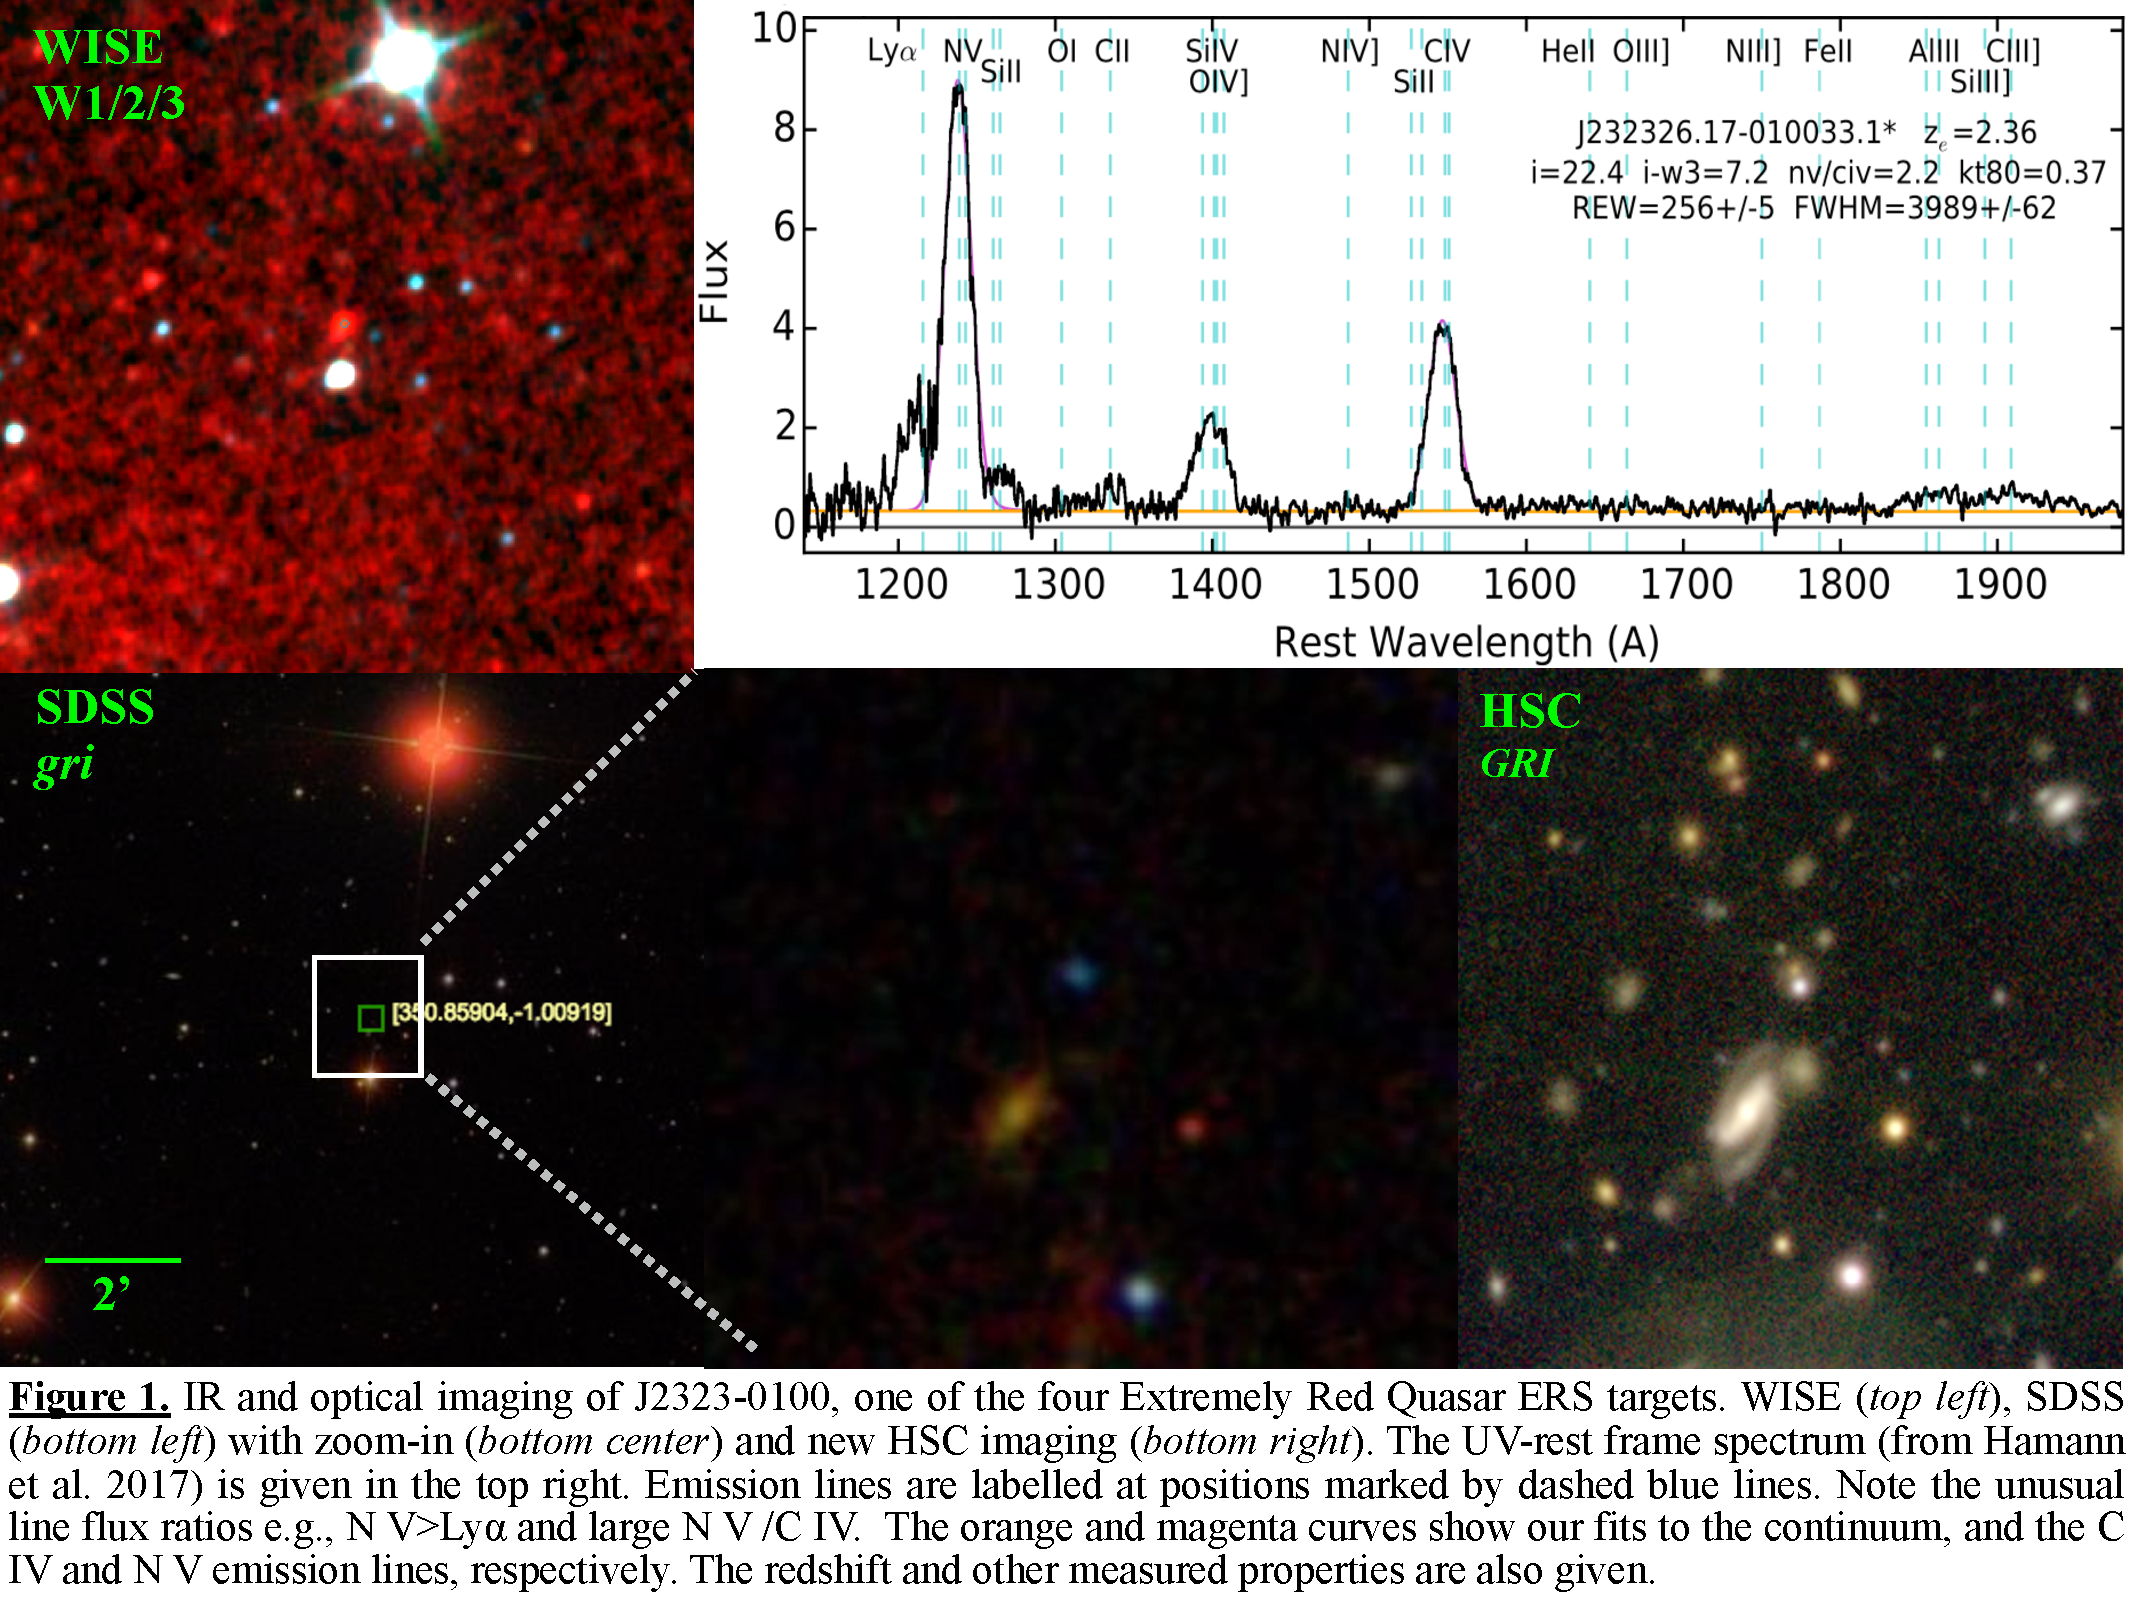
\includegraphics[]{WISE_SDSSzoomHSC_ERQ-image_v2.pdf}
    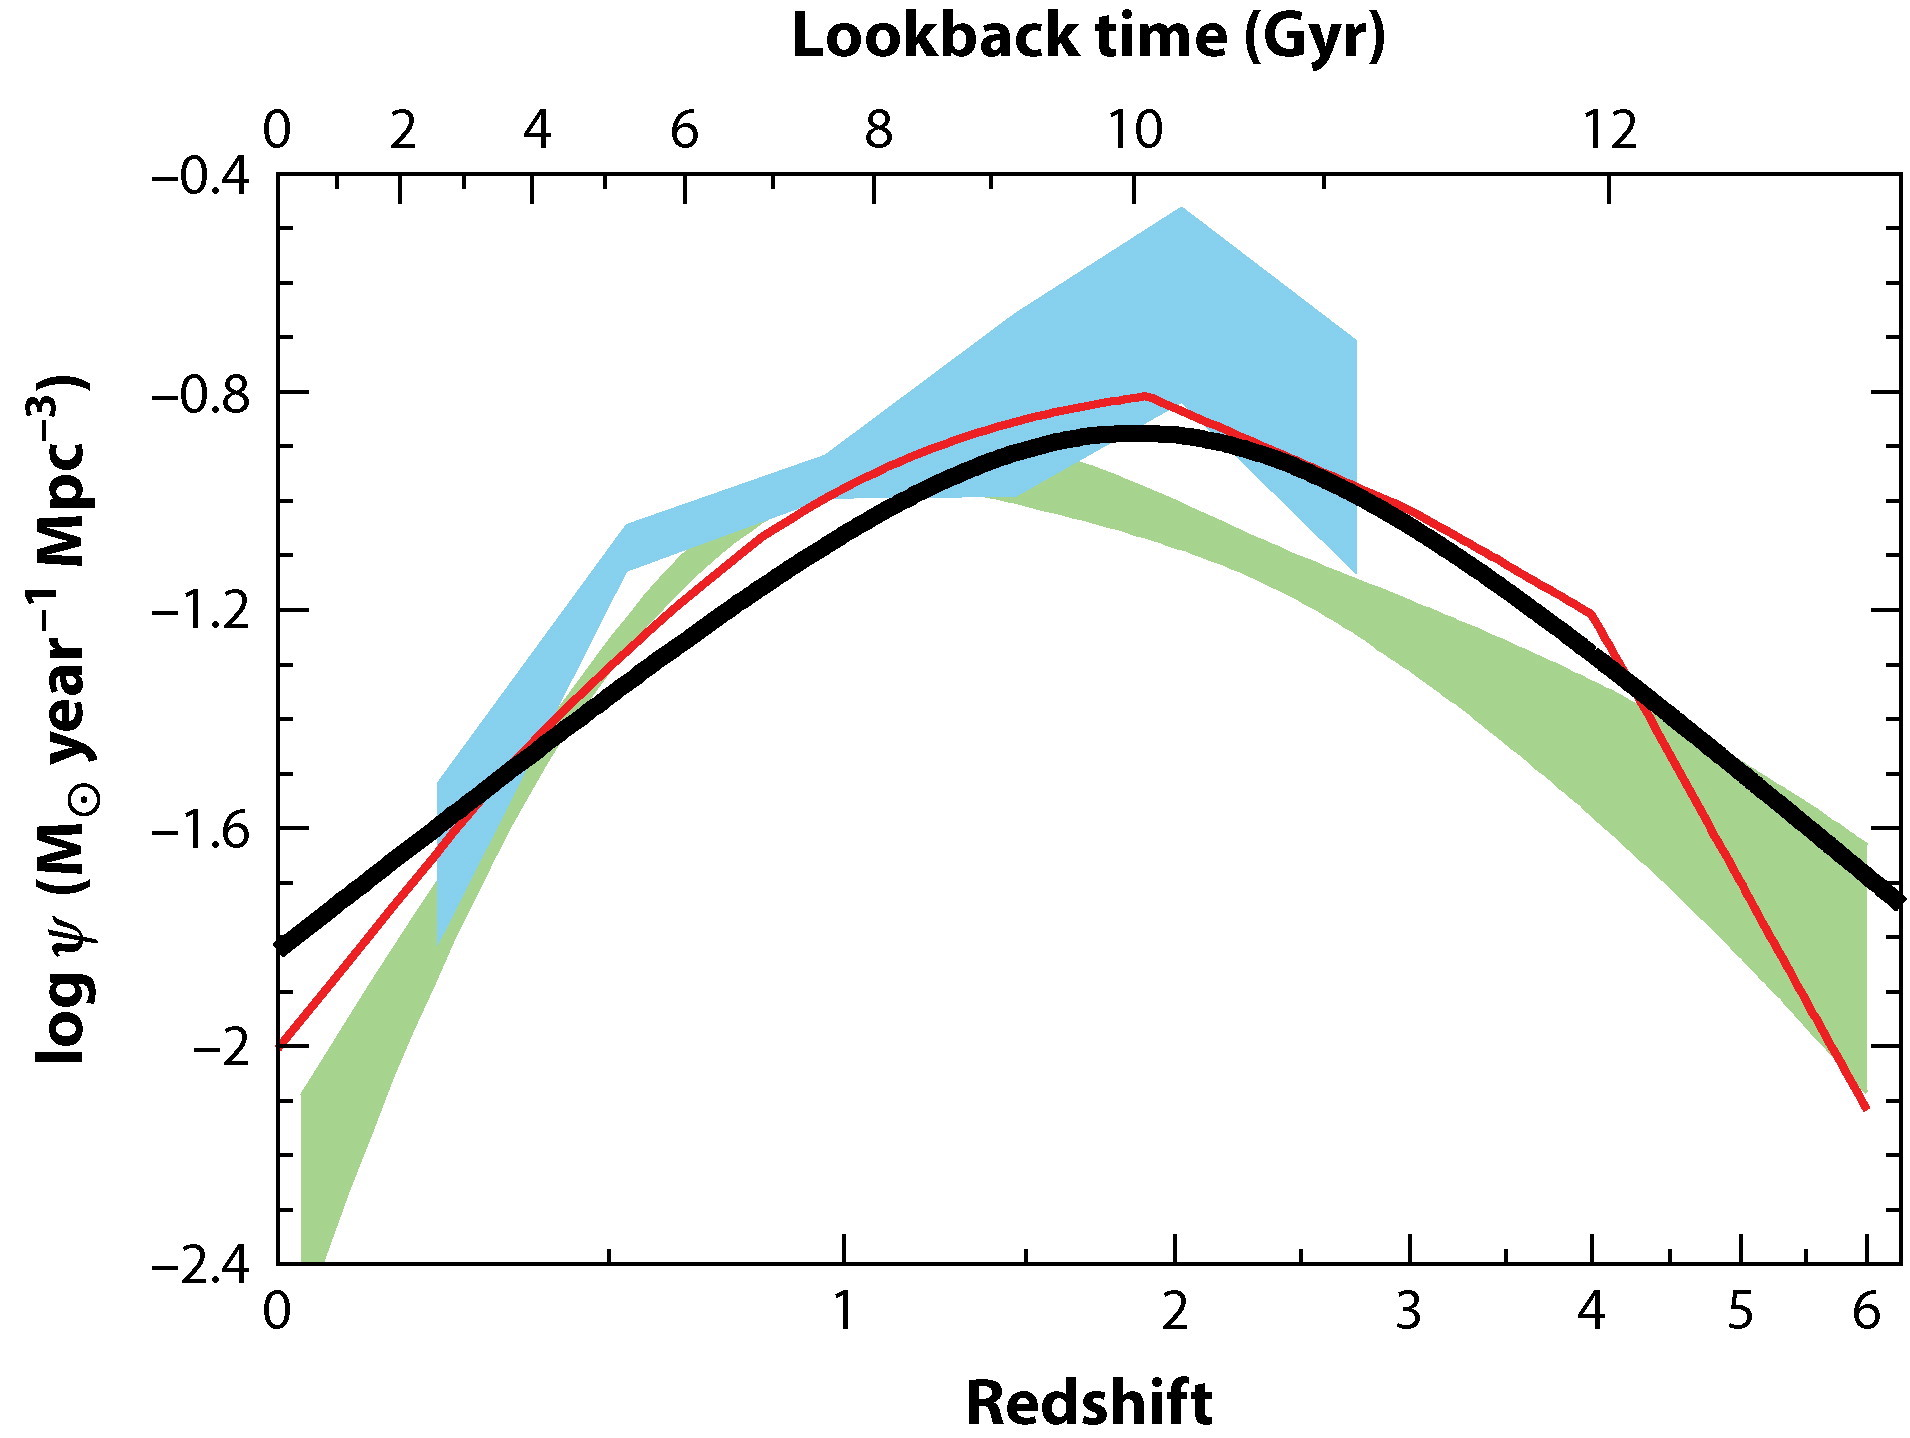
\includegraphics[height=12.0cm,width=16.0cm]{../Figures/MadauDickinson2014_Fig15_hires.jpeg}
    \vspace{-10pt}
\caption{Figure 15 from Madau \& Dickinson (2014):   
 Comparison of the best-fit star-formation history (thick solid curve)
with the massive black hole accretion history from X-ray [red curve
(Shankar et al. 2009); light green shading (Aird et al. 2010)] and
infrared (light blue shading) (Delvecchio et al. 2014) data. The
shading indicates the $\pm1\sigma$ uncertainty range on the total
bolometric luminosity density. The radiative efficiency has been set
to $\epsilon = 0.1$. The comoving rates of black hole accretion have been
scaled up by a factor of 3,300 to facilitate visual comparison to the
star-formation history.}
    \label{figtest-fig}
  \end{center}
\end{figure}



%%%%%%%%%%%%%%%%%%%%%%%%%%%%%%%%%%%%%%%%%%%%%%%%%%%%%%%%%%%%%%%%%%%%%%%%%%%

%   2. TECHNICAL JUSTIFICATION
%       (see https://jwst-docs.stsci.edu/display/JSP/JWST+Cycle+1+Proposal+Preparation)
%
%
\justifyobservations   % Do not delete this command.
% Enter your description of the observations.
%%%%%%%%%%%%%%%%%%%%%%%%%%%%%%%%%%%%%%%%%%%%%%
%%
%%    D e s c r i p t i o n    o f     t h e      O b s e r v a t i o n s  : 
%%
%%%%%%%%%%%%%%%%%%%%%%%%%%%%%%%%%%%%%%%%%%%%%%

\hspace{-7.5cm}
\begin{figure}[h]
  \begin{center}
    \hspace{-0.5cm}
%    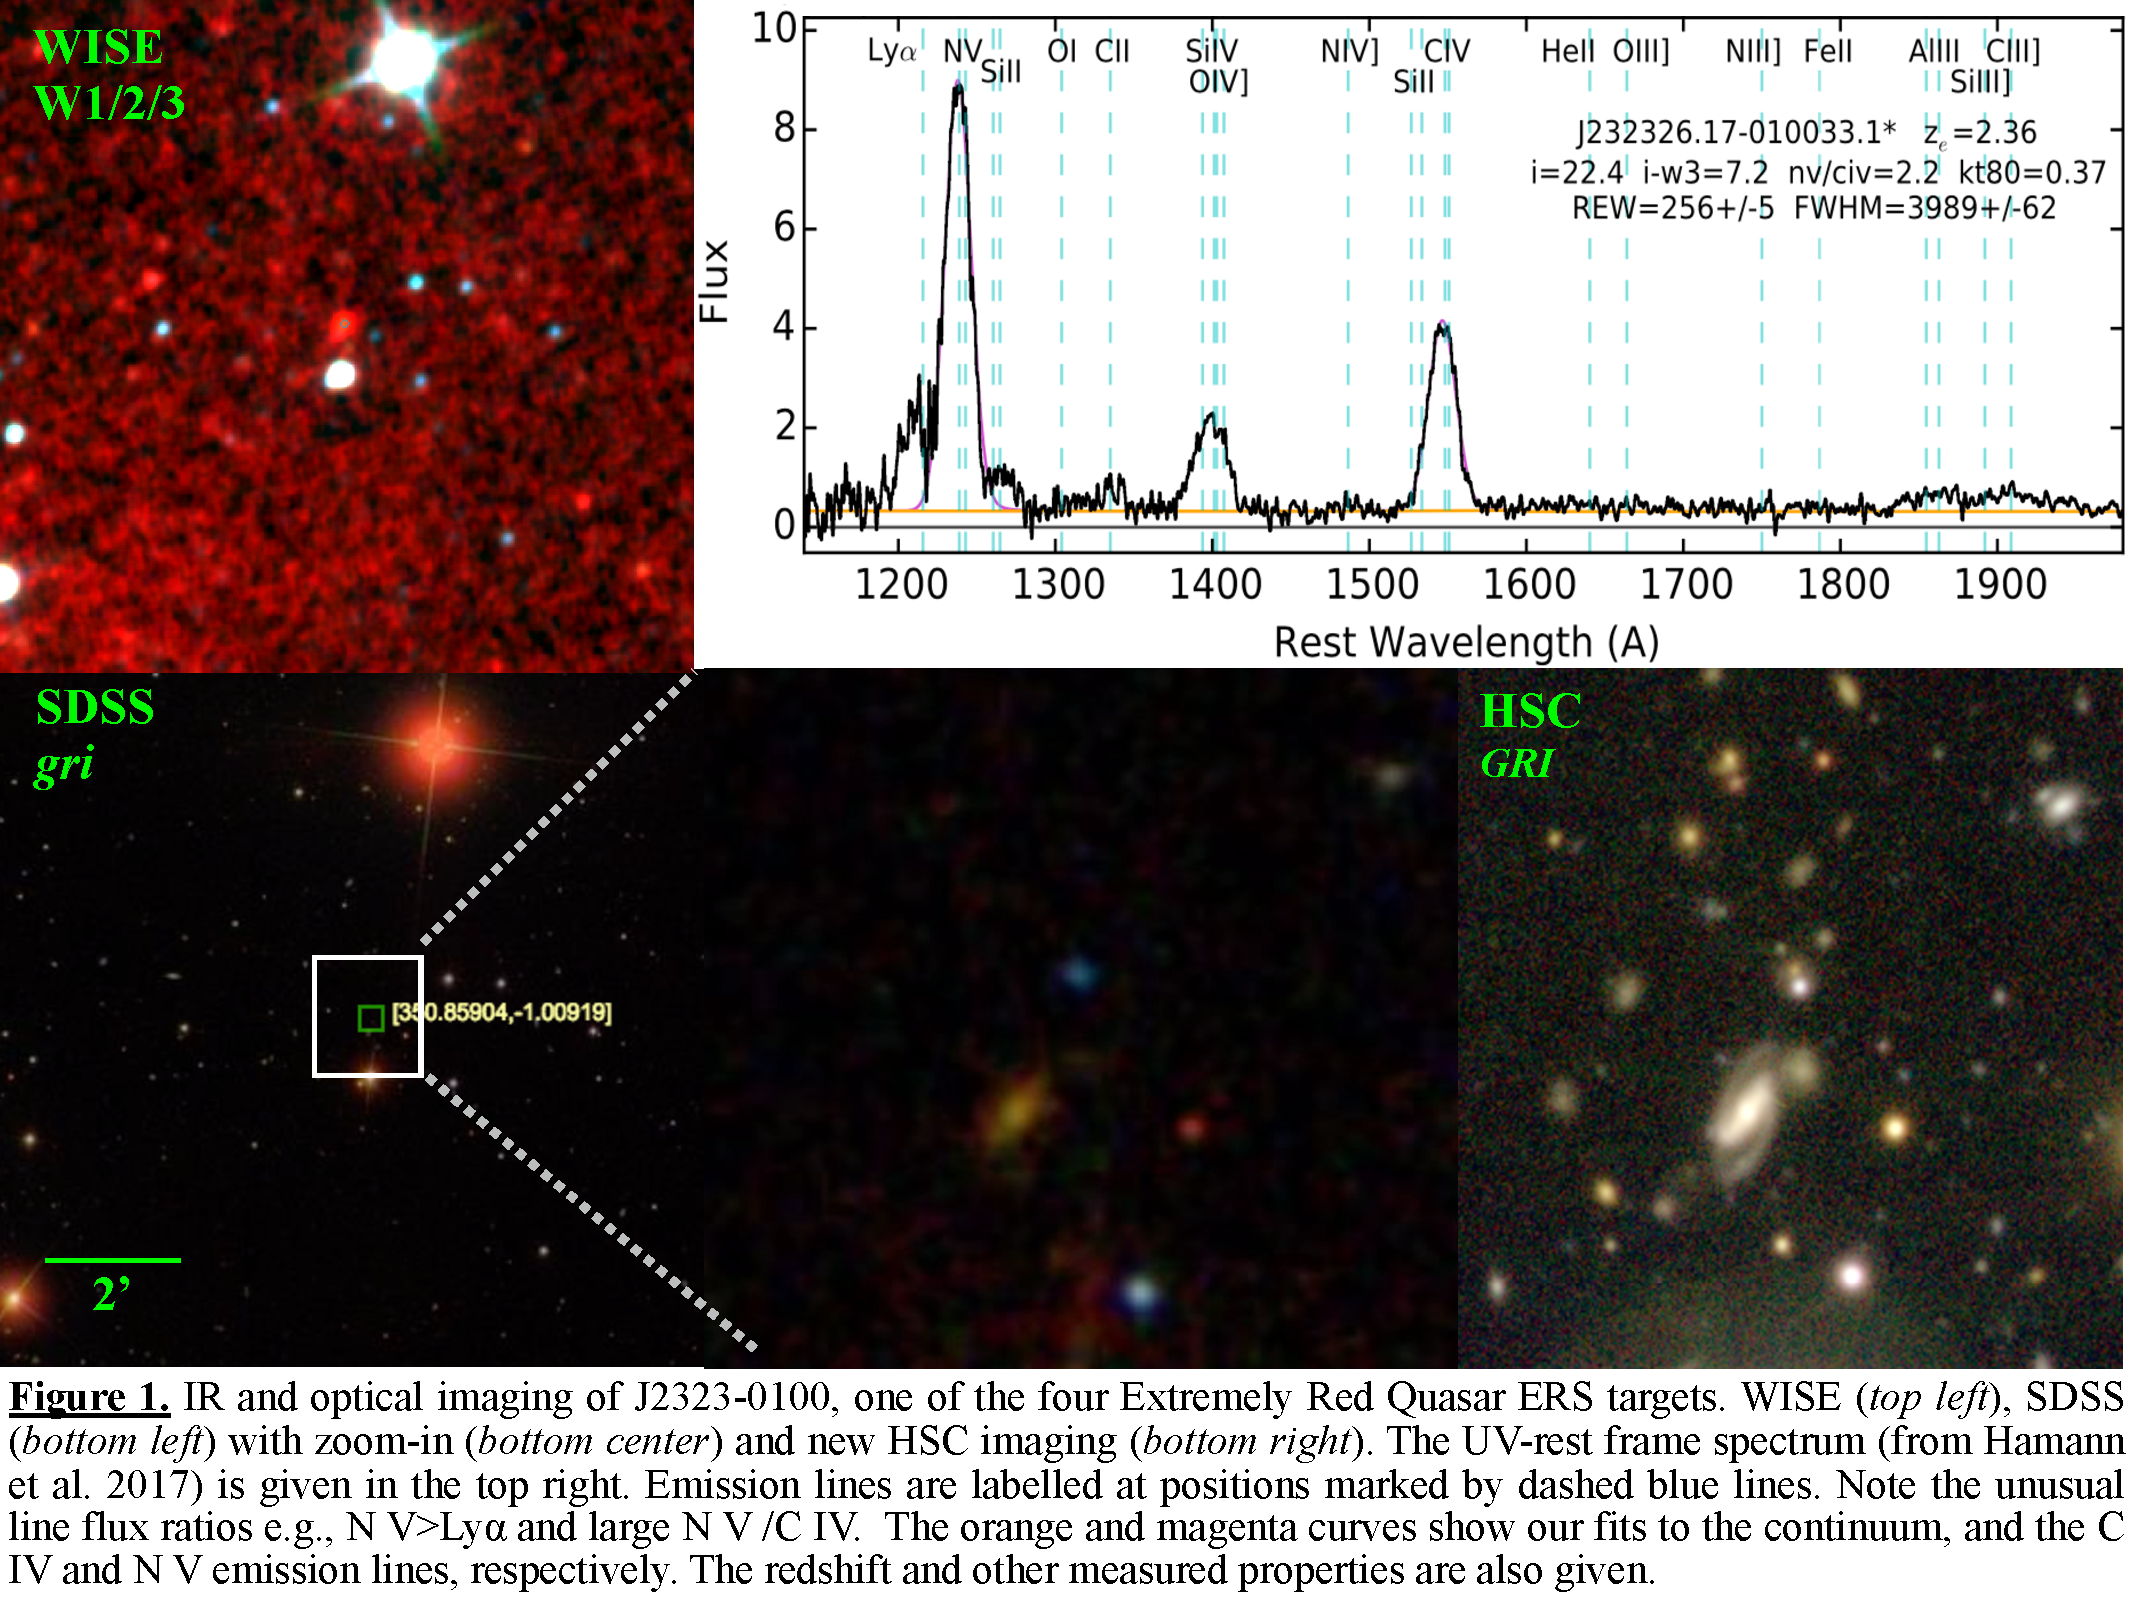
\includegraphics[]{WISE_SDSSzoomHSC_ERQ-image_v2.pdf}
    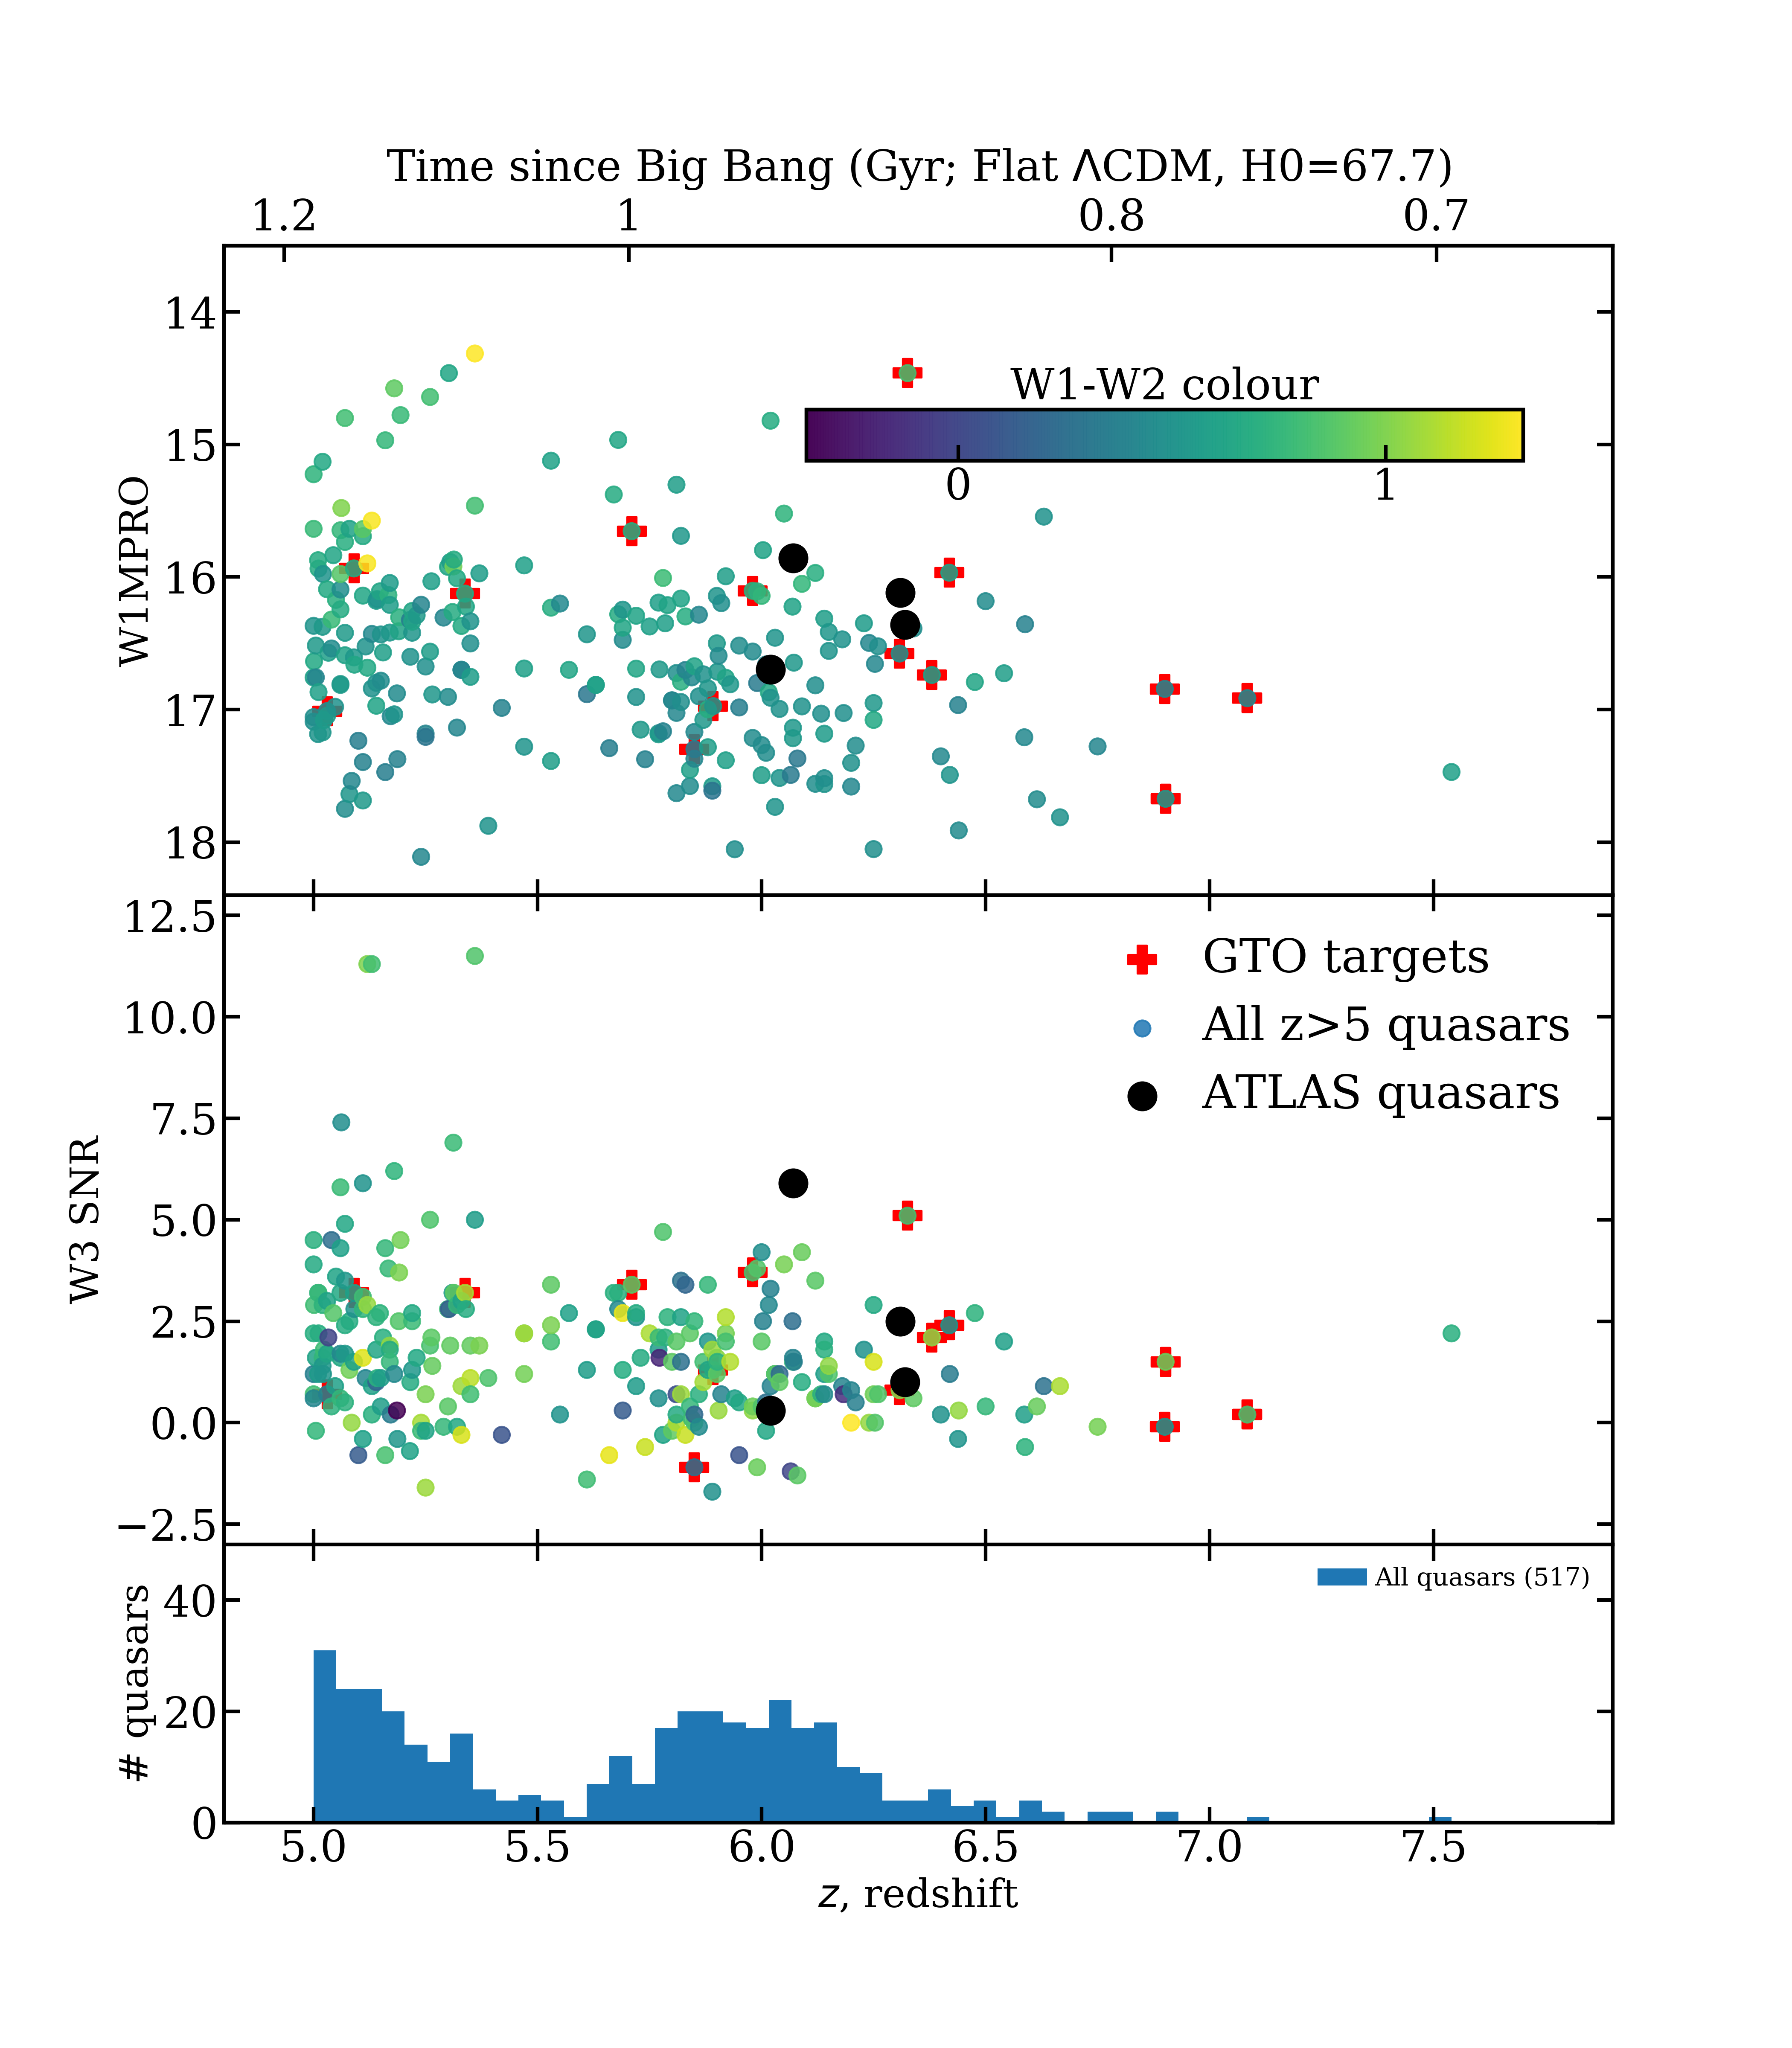
\includegraphics[height=14.0cm,width=12.0cm]{W1W2_vs_redshift_20180308v1.png}
    \vspace{-10pt}
\caption{Ned Wright's talk; 
https://www.ipac.caltech.edu/exgal2011/sched.shtml}
    \label{figtest-fig}
  \end{center}
\end{figure}



%%%%%%%%%%%%%%%%%%%%%%%%%%%%%%%%%%%%%%%%%%%%%%%%%%%%%%%%%%%%%%%%%%%%%%%%%%%

%   2a. SPECIAL REQUIREMENTS
%        (see https://jwst-docs.stsci.edu/display/JSP/JWST+Cycle+1+Proposal+Preparation)
%
%
\specialreq             % Do not delete this command.
% Justify your special requirements here, if any.



%%%%%%%%%%%%%%%%%%%%%%%%%%%%%%%%%%%%%%%%%%%%%%%%%%%%%%%%%%%%%%%%%%%%%%%%%%%

%   2b. COORDINATED PARALLEL OBSERVATIONS
%        (see https://jwst-docs.stsci.edu/display/JSP/JWST+Cycle+1+Proposal+Preparation)
%
%
\coordinatedobs % Do not delete this command.
% Enter your coordinated parallel observing plans here, if any.

%%%%%%%%%%%%%%%%%%%%%%%%%%%%%%%%%%%%%%%%%%%%%%%%%%%%%%%%%%%%%%%%%%%%%%%%%%%

%   2c. JUSTIFY DUPLICATIONS
%        (see https://jwst-docs.stsci.edu/display/JSP/JWST+Cycle+1+Proposal+Preparation)
%
%
\duplications           % Do not delete this command.
% Enter your duplication justifications here, if any.

%%%%%%%%%%%%%%%%%%%%%%%%%%%%%%%%%%%%%%%%%%%%%%%%%%%%%%%%%%%%%%%%%%%%%%%%%%%

%   3. DATA PROCESSING AND ANALYSIS PLAN
%       (see https://jwst-docs.stsci.edu/display/JSP/JWST+Cycle+1+Proposal+Preparation)
%
%
\analysisplan % Do not delete this command.
% Describe the data processing and analysis plan here.

%%%%%%%%%%%%%%%%%%%%%%%%%%%%%%%%%%%%%%%%%%%%%%%%%%%%%%%%%%%%%%%%%%%%%%%%%%%

%   4. Management Plan
%       (see https://jwst-docs.stsci.edu/display/JSP/JWST+Cycle+1+Proposal+Preparation)
%
%
\managementplan % Do not delete this command.
% Describe the data processing and analysis plan here.

%%%%%%%%%%%%%%%%%%%%%%%%%%%%%%%%%%%%%%%%%%%%%%%%%%%%%%%%%%%%%%%%%%%%%%%%%%%




\end{document}          % End of proposal. Do not delete this line.
                        % Everything after this command is ignored.

